%
% Complete documentation on the extended LaTeX markup used for Insight
% documentation is available in ``Documenting Insight'', which is part
% of the standard documentation for Insight.  It may be found online
% at:
%
%     http://www.itk.org/

\documentclass{InsightArticle}


%%%%%%%%%%%%%%%%%%%%%%%%%%%%%%%%%%%%%%%%%%%%%%%%%%%%%%%%%%%%%%%%%%
%
%  hyperref should be the last package to be loaded.
%
%%%%%%%%%%%%%%%%%%%%%%%%%%%%%%%%%%%%%%%%%%%%%%%%%%%%%%%%%%%%%%%%%%
\usepackage[dvips,
bookmarks,
bookmarksopen,
backref,
colorlinks,linkcolor={blue},citecolor={blue},urlcolor={blue},
]{hyperref}
% to be able to use options in graphics
\usepackage{graphicx}
% for pseudo code
\usepackage{listings}
% subfigures
\usepackage{subfigure}


%  This is a template for Papers to the Insight Journal. 
%  It is comparable to a technical report format.

% The title should be descriptive enough for people to be able to find
% the relevant document. 
\title{Minimal Path Image Filter}

% Increment the release number whenever significant changes are made.
% The author and/or editor can define 'significant' however they like.
\release{0.00}

% At minimum, give your name and an email address.  You can include a
% snail-mail address if you like.
\author{Richard Beare}
\authoraddress{Richard.Beare@med.monash.edu.au}

\begin{document}
\maketitle

\ifhtml
\chapter*{Front Matter\label{front}}
\fi


\begin{abstract}
\noindent
The Dijkstra-Moore minimal path algorithm has applications in image
analysis for finding markers between defined endpoints or following
linear structures. This document instroduces a filter that computes
the minimal path between markers in an image and returns an image of
the path.
\end{abstract}

\tableofcontents

\section{Introduction}
The minimal path algorithm from graph theory is well known and won't
be described here.

Minimal paths have a number of applications in image analysis - for
example following irregular shaped features or tracking edges. The
resulting path will be continuous and a single pixel thick. The
algorithm will work on images of any dimension, but the path will
always be one pixel thick - i.e. if you apply to 3D images you won't
compute a minimal surface.

In this filter the cost of a path is a combination of the distance
between adjacent voxels and the voxel brightness. The distance between
adjacent voxels is computed using spacing information and can
therefore deal with non cubic voxels. Distances between diagonal
pixels are also taken into account. The cost of a path reaching step
$i$ is $C_i = C_{i-1} + (1+ B(i)) * d(i,i-1)$. This notation is a bit
dodgy, with step number and coordinates both being represented by $i$,
so $B(i)$ is the brightness at location $i$ and $d(i, i-1)$ is the
distance between neighbouring steps in the path. The $1$ is included
so that there is some cost in moving across blank areas. 

\section{Minimal Path Image Filter interface and examples}
The new filter is called {\em itkMinimalPathImageFilter} and is
templated over an input image type and a label image type. The result
is a label image. The path is painted in the label image with either
the first label or label defined by the user. Future versions may
return a path structure of the formed used elsewhere in ITK. 

The user controls are:
\begin{itemize}
\item {\bf FullyConnected} - defines whether the path should be face 
connected or should be able to cross diagonals.
\item {\bf Direction} - defines a dominant direction - e.g x,y,z. 
The filter then uses the location of the markers to figure out the
sign of the direction. The FullyConnected option is redundant if
direction is set. By default the direction is not constrained, which
means that the path can double back on itself (but not cross,
naturally). If the direction is constrained by setting this value then
the path can only take steps with components in the direction
defined. It is therefore possible to create start and end points that
cannot be reached based on these constraints, so care must be
taked. For example, if we define a left to right path (direction = 0),
and place the start marker in the top left corner and the end marker
in the bottom right, there will be no valid path if the image has more
pixels in the vertical than horizontal direction because the path can
only move downwards at 45 degrees.
\item {\bf StartLabel, EndLabel} - defines the labels used to mark the 
start and end of the path.
\item {\bf MarkLabel} - defines the label in which the computed path 
will be marked.
\item {\bf LabelChain} - a vector of labels to define links in a path. 
These links can be circular, but sections of path are computed
independently and may therefore cross.
\item {\bf UnitCost} - is the base cost for crossing a pixel. It is one 
by default to make the cost of crossing blank pixels
positive. Increasing this should bias the cost function towards the
length of the path rather than the brightness of pixels on it.
\end{itemize}

The cost of the final path(s) may be queried with the {\bf GetCost} method.

\subsection{Examples}
These examples may be created by running the test program distributed with this package.

Figure \ref{fig:basicPath} illustrates a simple example of a minimal
path between two user defined endpoints. The resulting path follows
the dark region and could be used to create a marker for further
processing. Figure \ref{fig:basicPathB} illustrates the minimal path
between the same endpoints through the orginal image. The path seeks
the part of the image that has been set to zero by the rotation of the
image, which is why the path is so far from the edge of the
head. Figure \ref{fig:basicPathM} shows an example of multiple paths
forming a closed loop.

\begin{figure}[htbp]
\begin{center}
\subfigure[Markers on inverted cthead]{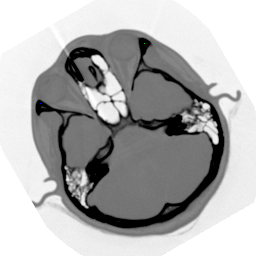
\includegraphics[scale=0.5]{basicPathMarker}\label{fig:basicPathMarker}}
\subfigure[Computed path]{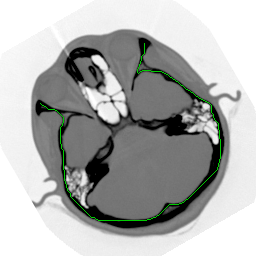
\includegraphics[scale=0.5]{basicPathOv}\label{fig:basicPathOv}}
\caption{Minimal path through inverted cthead from user defined endpoints.\label{fig:basicPath}}
\end{center}
\end{figure}

\begin{figure}[htbp]
\begin{center}
\subfigure[Markers on cthead]{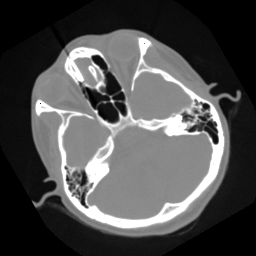
\includegraphics[scale=0.5]{basicPathBMarker}\label{fig:basicPathBMarker}}
\subfigure[Computed path]{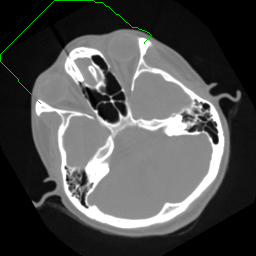
\includegraphics[scale=0.5]{basicPathBOv}\label{fig:basicPathBOv}}
\caption{Minimal path through cthead from user defined endpoints.\label{fig:basicPathB}}
\end{center}
\end{figure}

\begin{figure}[htbp]
\begin{center}
\subfigure[Markers on cthead]{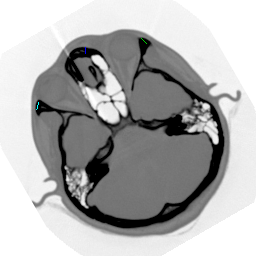
\includegraphics[scale=0.5]{basicPathMMarker}\label{fig:basicPathMMarker}}
\subfigure[Computed path]{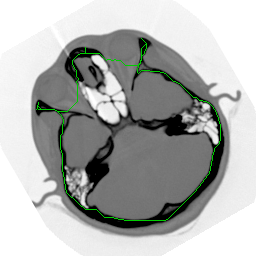
\includegraphics[scale=0.5]{basicPathMOv}\label{fig:basicPathMOv}}
\caption{Minimal paths through inverted cthead so that the result is a closed loop.\label{fig:basicPathM}}
\end{center}
\end{figure}


\begin{figure}[htbp]
\centering
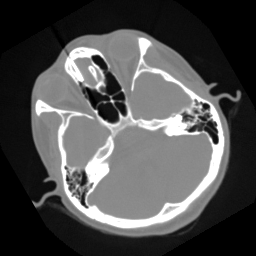
\includegraphics{cthead1}
\caption{The input image.\label{cthead1}}
\end{figure}





\bibliographystyle{plain}
\bibliography{InsightJournal}
\nocite{ITKSoftwareGuide}

\end{document}

